\documentclass[11pt,a4paper]{report}
\usepackage[textwidth=37em,vmargin=30mm]{geometry}
\usepackage{calc,xunicode,amsmath,amssymb,paralist,enumitem,tabu,booktabs,datetime2,xeCJK,xeCJKfntef,listings}
\usepackage{tocloft,fancyhdr,tcolorbox,xcolor,graphicx,eso-pic,xltxtra,xelatexemoji}

\newcommand{\envyear}[0]{2025}
\newcommand{\envdatestr}[0]{2025-03-29}
\newcommand{\envfinaldir}[0]{webdb/2025/20250329/final}

\usepackage[hidelinks]{hyperref}
\hypersetup{
    colorlinks=false,
    pdfpagemode=FullScreen,
    pdftitle={Web Digest - \envdatestr}
}

\setlength{\cftbeforechapskip}{10pt}
\renewcommand{\cftchapfont}{\rmfamily\bfseries\large\raggedright}
\setlength{\cftbeforesecskip}{2pt}
\renewcommand{\cftsecfont}{\sffamily\small\raggedright}

\setdefaultleftmargin{2em}{2em}{1em}{1em}{1em}{1em}

\usepackage{xeCJK,xeCJKfntef}
\xeCJKsetup{PunctStyle=plain,RubberPunctSkip=false,CJKglue=\strut\hskip 0pt plus 0.1em minus 0.05em,CJKecglue=\strut\hskip 0.22em plus 0.2em}
\XeTeXlinebreaklocale "zh"
\XeTeXlinebreakskip = 0pt


\setmainfont{Brygada 1918}
\setromanfont{Brygada 1918}
\setsansfont{IBM Plex Sans}
\setmonofont{JetBrains Mono NL}
\setCJKmainfont{Noto Serif CJK SC}
\setCJKromanfont{Noto Serif CJK SC}
\setCJKsansfont{Noto Sans CJK SC}
\setCJKmonofont{Noto Sans CJK SC}

\setlength{\parindent}{0pt}
\setlength{\parskip}{8pt}
\linespread{1.15}

\lstset{
	basicstyle=\ttfamily\footnotesize,
	numbersep=5pt,
	backgroundcolor=\color{black!5},
	showspaces=false,
	showstringspaces=false,
	showtabs=false,
	tabsize=2,
	captionpos=b,
	breaklines=true,
	breakatwhitespace=true,
	breakautoindent=true,
	linewidth=\textwidth
}






\newcommand{\coverpic}[2]{
    % argv: itemurl, authorname
    Cover photo by #2~~(\href{#1}{#1})
}
\newcommand{\makeheader}[0]{
    \begin{titlepage}
        % \newgeometry{hmargin=15mm,tmargin=21mm,bmargin=12mm}
        \begin{center}
            
            \rmfamily\scshape
            \fontspec{BaskervilleF}
            \fontspec{Old Standard}
            \fontsize{59pt}{70pt}\selectfont
            WEB\hfill DIGEST
            
            \vfill
            % \vskip 30pt
            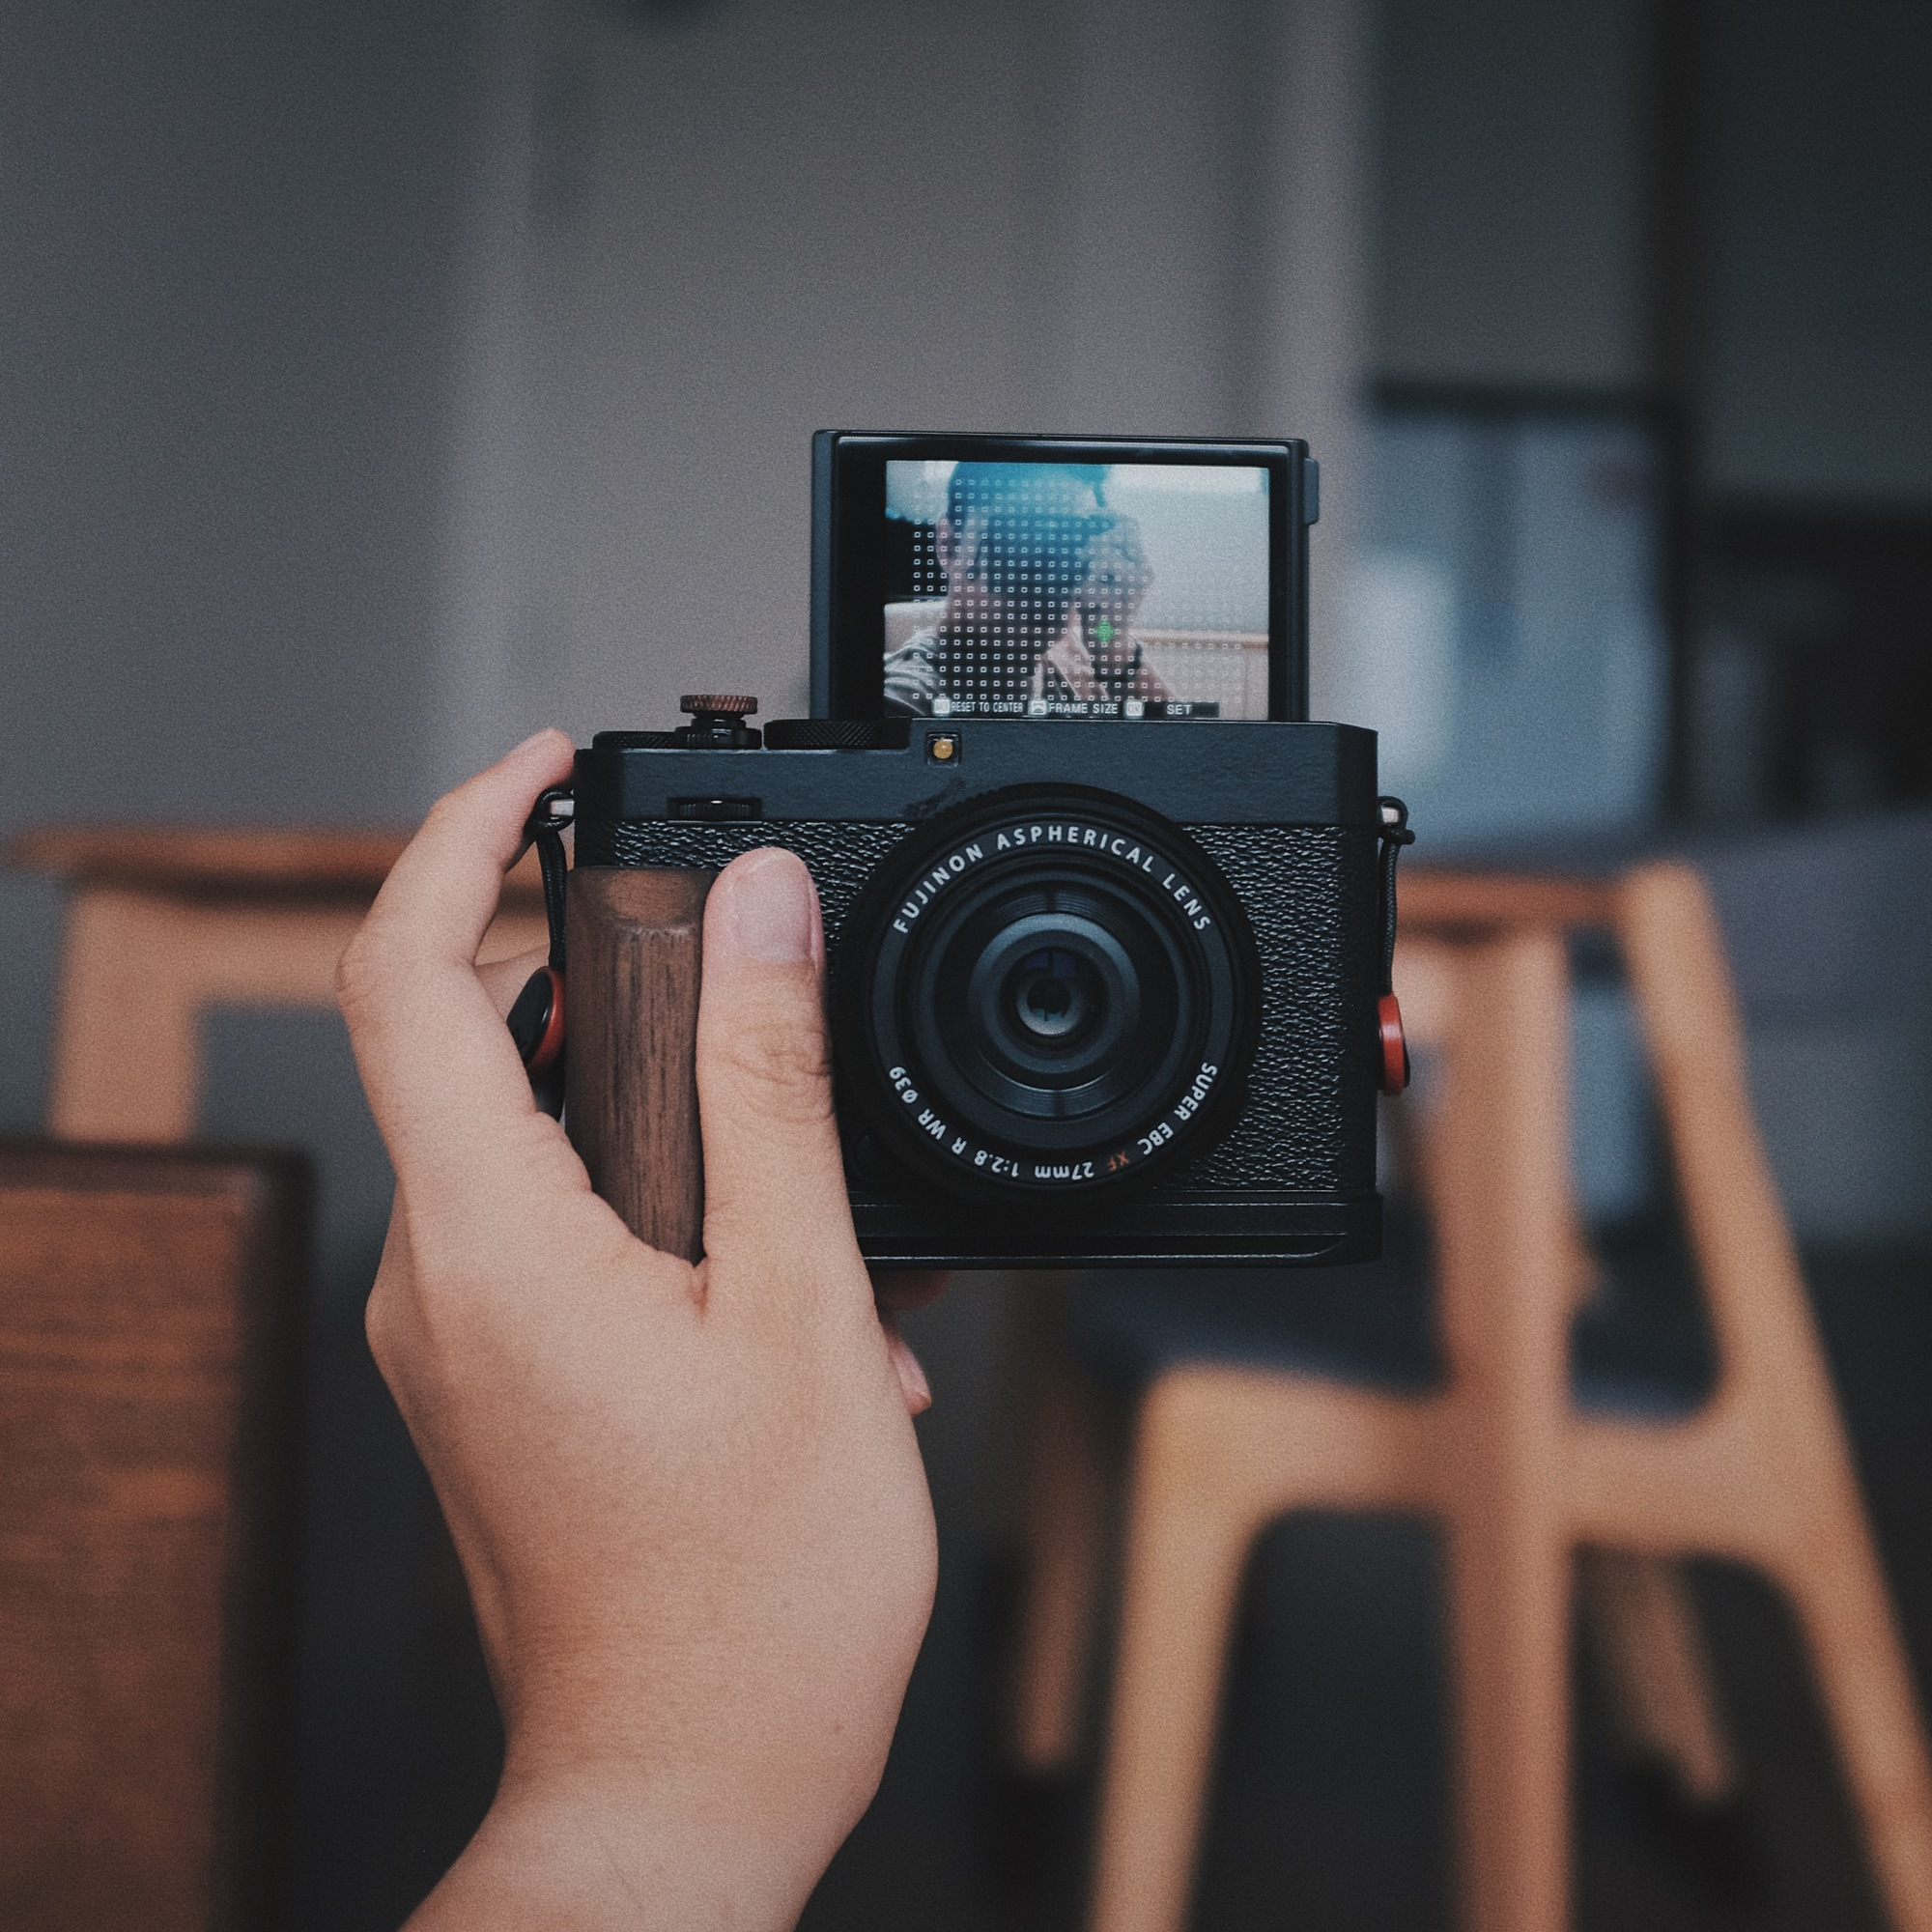
\includegraphics[width=\linewidth]{\envfinaldir/coverpic-prod.jpg}\par
            % \vskip 30pt
            \vfill

            \normalsize\rmfamily\scshape
            \copyright{} The Web Digest Project \hfill\large \envdatestr
        \end{center}
    \end{titlepage}
    % \restoregeometry
}
\newcommand{\simplehref}[1]{%
    \textcolor{blue!80!green}{\href{#1}{#1}}%
}
\renewcommand{\contentsname}{\center\Huge\sffamily\bfseries Contents\par\vskip 20pt}
\newcounter{ipartcounter}
\setcounter{ipartcounter}{0}
\newcommand{\ipart}[1]{
    % \vskip 20pt
    \clearpage
    \stepcounter{ipartcounter}
    \phantomsection
    \addcontentsline{toc}{chapter}{#1}
    % \begin{center}
    %     \Huge
    %     \sffamily\bfseries
    %     #1
    % \end{center}
    % \vskip 20pt plus 7pt
}
\newcounter{ichaptercounter}
\setcounter{ichaptercounter}{0}
\newcommand{\ichapter}[1]{
    % \vskip 20pt
    \clearpage
    \stepcounter{ichaptercounter}
    \phantomsection
    \addcontentsline{toc}{section}{\numberline{\arabic{ichaptercounter}}#1}
    \begin{center}
        \Huge
        \sffamily\bfseries
        #1
    \end{center}
    \vskip 20pt plus 7pt
}
\newcommand{\entrytitlefont}[1]{\subsection*{\raggedright\Large\sffamily\bfseries#1}}
\newcommand{\entryitemGeneric}[2]{
    % argv: title, url
    \parbox{\linewidth}{
        \entrytitlefont{#1}\par\vskip 5pt
        \footnotesize\ttfamily\mdseries
        \simplehref{#2}
    }\vskip 11pt plus 11pt minus 1pt
}
\newcommand{\entryitemGithub}[3]{
    % argv: title, url, desc
    \parbox{\linewidth}{
        \entrytitlefont{#1}\par\vskip 5pt
        \footnotesize\ttfamily\mdseries
        \simplehref{#2}\par\vskip 5pt
        \small\rmfamily\mdseries#3
    }\vskip 11pt plus 11pt minus 1pt
}
\newcommand{\entryitemAp}[3]{
    % argv: title, url, desc
    \parbox{\linewidth}{
        \entrytitlefont{#1}\par\vskip 5pt
        \footnotesize\ttfamily\mdseries
        \simplehref{#2}\par\vskip 5pt
        \small\rmfamily\mdseries#3
    }\vskip 11pt plus 11pt minus 1pt
}
\newcommand{\entryitemHackernews}[3]{
    % argv: title, hnurl, rawurl
    % \parbox{\linewidth}{
    %     \entrytitlefont{#1}\par\vskip 5pt
    %     \footnotesize\ttfamily\mdseries
    %     \simplehref{#3}\par
    %     \textcolor{black!50}{\href{#2}{#2}}
    % }\vskip 11pt plus 11pt minus 1pt
    \begin{minipage}{\linewidth}
            \entrytitlefont{#1}\par\vskip 5pt
            \footnotesize\ttfamily\mdseries
            \simplehref{#3}\par
            \textcolor{black!50}{\href{#2}{#2}}
    \end{minipage}\par\vskip 11pt plus 11pt minus 1pt
}







\begin{document}

\makeheader

\tableofcontents\clearpage




\ipart{Developers}
\ichapter{Hacker News}
\entryitemTwoLinks{2025 Tariff Impacts at Puget Systems}{https://news.ycombinator.com/item?id=43510870}{https://www.pugetsystems.com/blog/2025/03/28/2025-tariff-impacts-at-puget-systems/}

\entryitemTwoLinks{xAI has acquired X, xAI now valued at \$80B}{https://news.ycombinator.com/item?id=43509923}{https://twitter.com/elonmusk/status/1905731750275510312}

\entryitemTwoLinks{We hacked Gemini's Python sandbox and leaked its source code (at least some)}{https://news.ycombinator.com/item?id=43508418}{https://www.landh.tech/blog/20250327-we-hacked-gemini-source-code/}

\entryitemTwoLinks{How Kerala got rich}{https://news.ycombinator.com/item?id=43507286}{https://aeon.co/essays/how-did-kerala-go-from-poor-to-prosperous-among-indias-states}

\entryitemTwoLinks{Decomposing a Factorial into Large Factors}{https://news.ycombinator.com/item?id=43506238}{https://terrytao.wordpress.com/2025/03/26/decomposing-a-factorial-into-large-factors/}

\entryitemTwoLinks{The Biology of a Large Language Model}{https://news.ycombinator.com/item?id=43505748}{https://transformer-circuits.pub/2025/attribution-graphs/biology.html}

\entryitemTwoLinks{Despite Ukraine war, Europe imported even more Russian gas last year}{https://news.ycombinator.com/item?id=43505700}{https://e360.yale.edu/digest/europe-russia-ukraine-war-natural-gas-2024}

\entryitemTwoLinks{Japanese scientists create new plastic that dissolves in saltwater overnight}{https://news.ycombinator.com/item?id=43505626}{https://newatlas.com/materials/plastic-dissolves-ocean-overnight-no-microplastics/}

\entryitemTwoLinks{Getting hit by lightning is good for some tropical trees}{https://news.ycombinator.com/item?id=43505447}{https://www.caryinstitute.org/news-insights/press-release/getting-hit-lightning-good-some-tropical-trees}

\entryitemTwoLinks{Cross-Platform P2P Wi-Fi: How the EU Killed AWDL}{https://news.ycombinator.com/item?id=43505022}{https://www.ditto.com/blog/cross-platform-p2p-wi-fi-how-the-eu-killed-awdl}

\entryitemTwoLinks{Are Levi's from Amazon different from Levi's from Levi's?}{https://news.ycombinator.com/item?id=43504451}{https://nymag.com/strategist/article/levis-amazon-jeans-testing.html}

\entryitemTwoLinks{I asked police to send me their public surveillance footage of my car}{https://news.ycombinator.com/item?id=43504413}{https://cardinalnews.org/2025/03/28/i-drove-300-miles-in-rural-virginia-then-asked-police-to-send-me-their-public-surveillance-footage-of-my-car-heres-what-i-learned/}

\entryitemTwoLinks{How to write blog posts that developers read}{https://news.ycombinator.com/item?id=43503872}{https://refactoringenglish.com/chapters/write-blog-posts-developers-read/}

\entryitemTwoLinks{Google is publishing the home addresses of developers without their consent}{https://news.ycombinator.com/item?id=43503720}{https://news.ycombinator.com/item?id=43503720}

\entryitemTwoLinks{Learn to code, ignore AI, then use AI to code even better}{https://news.ycombinator.com/item?id=43503295}{https://kyrylo.org/software/2025/03/27/learn-to-code-ignore-ai-then-use-ai-to-code-even-better.html}

\entryitemTwoLinks{7.7 magnitude earthquake hits Southeast Asia, affecting Myanmar and Thailand}{https://news.ycombinator.com/item?id=43503265}{https://twitter.com/TaraBull808/status/1905534938558157139}

\entryitemTwoLinks{Xee: A Modern XPath and XSLT Engine in Rust}{https://news.ycombinator.com/item?id=43502291}{https://blog.startifact.com/posts/xee/}

\entryitemTwoLinks{Architecture Patterns with Python}{https://news.ycombinator.com/item?id=43501989}{https://www.cosmicpython.com/book/preface.html}

\entryitemTwoLinks{Signal Chat Leak Angers U.S. Military Pilots}{https://news.ycombinator.com/item?id=43501821}{https://www.nytimes.com/2025/03/27/us/politics/pilots-signal-leak.html}

\entryitemTwoLinks{A decompilation and port of Sonic Advance 2-a GameBoy Advance game written in C}{https://news.ycombinator.com/item?id=43500769}{https://github.com/SAT-R/sa2}\ichapter{Phoronix}
\entryitemGeneric{\hskip 0pt{}Linux 6.15 Graphics Drivers: NOVA Core, Apple Touch Bar, Lots For AMD + Intel GPUs}{https://www.phoronix.com/news/Linux-6.15-DRM-Graphics-Drivers}

\entryitemGeneric{\hskip 0pt{}GNOME 48 \& KDE Plasma 6.3 Delivering Great Wayland Desktop Experience On Ubuntu 25.04 For Linux Gaming}{https://www.phoronix.com/review/ubuntu-2504-kde-gnome-way}

\entryitemGeneric{\hskip 0pt{}Linux 6.15 Landing Backlight Driver For Various Apple iPhones \& iPads}{https://www.phoronix.com/news/Linux-6.15-Backlight-Apple}

\entryitemGeneric{\hskip 0pt{}Linux 6.15 Networking Delivers Many Nice Performance Optimizations \& New Hardware}{https://www.phoronix.com/news/Linux-6.15-Networking}

\entryitemGeneric{\hskip 0pt{}Linux Flips Around Its Behavior For Spectre-BHB Handling On ARM64}{https://www.phoronix.com/news/Linux-6.15-ARM64-Changes}

\entryitemGeneric{\hskip 0pt{}Ubuntu Provides More Insight Into Their Decision Not To "-O3" Optimize All Packages}{https://www.phoronix.com/news/Ubuntu-Details-No-O3-Everywhere}

\entryitemGeneric{\hskip 0pt{}Two Years In The Making, Intel Linux Driver Enables CPS Compression For Alchemist GPUs}{https://www.phoronix.com/news/Intel-CPS-Compression-Mesa}

\entryitemGeneric{\hskip 0pt{}Linux 6.15 Better Handles PS5 Controllers, AMD Human Presence Detection Off By Default}{https://www.phoronix.com/news/Linux-6.15-HID}

\entryitemGeneric{\hskip 0pt{}Nova DRM Skeleton Patches Further Flesh Out This Open-Source NVIDIA Kernel Driver}{https://www.phoronix.com/news/Nova-DRM-Skeleton-Driver-Patch}\ichapter{Dribbble}
\entryitemGeneric{\hskip 0pt{}The Rocky token landing page}{https://dribbble.com/shots/25827682-The-Rocky-token-landing-page}

\entryitemGeneric{\hskip 0pt{}Suffo - Real Estate Landing page Animation}{https://dribbble.com/shots/25829238-Suffo-Real-Estate-Landing-page-Animation}

\entryitemGeneric{\hskip 0pt{}Big gestures}{https://dribbble.com/shots/25826632-Big-gestures}

\entryitemGeneric{\hskip 0pt{}Proven UI/UX design, User Interface experience}{https://dribbble.com/shots/25819444-Proven-UI-UX-design-User-Interface-experience}

\entryitemGeneric{\hskip 0pt{}Dog + Play Button}{https://dribbble.com/shots/25809362-Dog-Play-Button}

\entryitemGeneric{\hskip 0pt{}Pricefy Logo Design - Mountains, Chart, Graph, Sun}{https://dribbble.com/shots/25824720-Pricefy-Logo-Design-Mountains-Chart-Graph-Sun}

\entryitemGeneric{\hskip 0pt{}Yada Yada Yada}{https://dribbble.com/shots/25826541-Yada-Yada-Yada}

\entryitemGeneric{\hskip 0pt{}Illustration}{https://dribbble.com/shots/25822720-Illustration}

\entryitemGeneric{\hskip 0pt{}Crypto Portfolio Tracker App}{https://dribbble.com/shots/25820014-Crypto-Portfolio-Tracker-App}

\entryitemGeneric{\hskip 0pt{}Gemini Rebrand}{https://dribbble.com/shots/25821410-Gemini-Rebrand}

\entryitemGeneric{\hskip 0pt{}Cyber Extrusion (Merch/Custom T-shirt)}{https://dribbble.com/shots/25821987-Cyber-Extrusion-Merch-Custom-T-shirt}

\entryitemGeneric{\hskip 0pt{}FCKD - Part 2}{https://dribbble.com/shots/25817864-FCKD-Part-2}

\entryitemGeneric{\hskip 0pt{}ROOT BEER}{https://dribbble.com/shots/25815759-ROOT-BEER}

\entryitemGeneric{\hskip 0pt{}Aura - Logo Design}{https://dribbble.com/shots/25815819-Aura-Logo-Design}

\entryitemGeneric{\hskip 0pt{}Complexure}{https://dribbble.com/shots/25815646-Complexure}

\entryitemGeneric{\hskip 0pt{}Snitcher - New Branding}{https://dribbble.com/shots/25816140-Snitcher-New-Branding}

\entryitemGeneric{\hskip 0pt{}Lepisov Branding Logo Reveal Animation}{https://dribbble.com/shots/25814536-Lepisov-Branding-Logo-Reveal-Animation}

\entryitemGeneric{\hskip 0pt{}Spark illustrations}{https://dribbble.com/shots/25815705-Spark-illustrations}

\entryitemGeneric{\hskip 0pt{}FCKD}{https://dribbble.com/shots/25812257-FCKD}

\entryitemGeneric{\hskip 0pt{}Spark}{https://dribbble.com/shots/25815686-Spark}

\entryitemGeneric{\hskip 0pt{}Spark illustrations}{https://dribbble.com/shots/25815717-Spark-illustrations}

\entryitemGeneric{\hskip 0pt{}Cimet Merch Car Wrapp}{https://dribbble.com/shots/25710572-Cimet-Merch-Car-Wrapp}

\entryitemGeneric{\hskip 0pt{}Revobyte Logo Design - R Letter / Monogram / Blockchain}{https://dribbble.com/shots/25811483-Revobyte-Logo-Design-R-Letter-Monogram-Blockchain}

\entryitemGeneric{\hskip 0pt{}S}{https://dribbble.com/shots/25814436-S}


\ipart{Developers~~~~(zh-Hans)}
\ichapter{Solidot}
\entryitemGeneric{\hskip 0pt{}AI 数据中心太多了}{https://www.solidot.org/story?sid=80915}

\entryitemGeneric{\hskip 0pt{}哥伦比亚大学学生因 AI 面试编程作弊工具而被停学}{https://www.solidot.org/story?sid=80914}

\entryitemGeneric{\hskip 0pt{}Ubuntu 25.04 (Plucky Puffin) Beta 释出}{https://www.solidot.org/story?sid=80913}

\entryitemGeneric{\hskip 0pt{}微软用预加载加速 Microsoft Office 启动}{https://www.solidot.org/story?sid=80912}

\entryitemGeneric{\hskip 0pt{}数据揭示了佛罗里达州在超速驾驶执法中存在种族歧视}{https://www.solidot.org/story?sid=80911}

\entryitemGeneric{\hskip 0pt{}缅甸发生 7.9 级/M7.7 级地震}{https://www.solidot.org/story?sid=80910}

\entryitemGeneric{\hskip 0pt{}吉卜力风格 AI 图像引版权争议}{https://www.solidot.org/story?sid=80909}

\entryitemGeneric{\hskip 0pt{}马的非凡耐力来自其基因突变}{https://www.solidot.org/story?sid=80908}

\entryitemGeneric{\hskip 0pt{}马斯克施压 Reddit CEO 去压制对其及 DOGE 的批评}{https://www.solidot.org/story?sid=80907}

\entryitemGeneric{\hskip 0pt{}Signal 在美国和也门的下载量大幅飙升}{https://www.solidot.org/story?sid=80906}

\entryitemGeneric{\hskip 0pt{}腾讯向育碧子公司投资 11.6 亿欧元}{https://www.solidot.org/story?sid=80905}

\entryitemGeneric{\hskip 0pt{}Valve 证实 Steam 简体中文玩家超过英语玩家}{https://www.solidot.org/story?sid=80904}

\entryitemGeneric{\hskip 0pt{}科学家建立女性怀孕前后身体变化图谱}{https://www.solidot.org/story?sid=80903}

\entryitemGeneric{\hskip 0pt{}跳槽不会再帮助你拿到更高的薪水}{https://www.solidot.org/story?sid=80902}

\entryitemGeneric{\hskip 0pt{}谁赢得了诺贝尔科学奖?}{https://www.solidot.org/story?sid=80901}

\entryitemGeneric{\hskip 0pt{}Meta 考虑在英国推出无广告的付费订阅}{https://www.solidot.org/story?sid=80900}

\entryitemGeneric{\hskip 0pt{}Vivaldi 内置 Proton VPN }{https://www.solidot.org/story?sid=80899}

\entryitemGeneric{\hskip 0pt{}VMware 指控西门子盗版了它的软件}{https://www.solidot.org/story?sid=80898}

\entryitemGeneric{\hskip 0pt{}日本数学家首次赢得阿贝尔奖}{https://www.solidot.org/story?sid=80897}

\entryitemGeneric{\hskip 0pt{}高盐饮食在小鼠诱发类抑郁症状}{https://www.solidot.org/story?sid=80895}\ichapter{V2EX}
\entryitemGeneric{\hskip 0pt{}[职场话题] 面试快 2 个月了,最终被迫去苏州了}{https://www.v2ex.com/t/1121886}

\entryitemGeneric{\hskip 0pt{}[宽带症候群] dae 透明代理如何启用 tproxy 模式}{https://www.v2ex.com/t/1121885}

\entryitemGeneric{\hskip 0pt{}[NAS] NAS 求推荐,绿联 DXP2800 vs 群晖 DS224+ (轻度使用+注重隐私)}{https://www.v2ex.com/t/1121883}

\entryitemGeneric{\hskip 0pt{}[创业组队] 一个 AI+的项目组队中,准备落地加拿大,一边创业,一边拿身份}{https://www.v2ex.com/t/1121882}

\entryitemGeneric{\hskip 0pt{}[玩家国度] 最近想新攒一台机子,配置如下,大家帮忙看看有没有问题?}{https://www.v2ex.com/t/1121881}

\entryitemGeneric{\hskip 0pt{}[远程工作] JS 全栈工程师 (远程)}{https://www.v2ex.com/t/1121879}

\entryitemGeneric{\hskip 0pt{}[问与答] 突发奇想,技术上有没有办法让多个企业共用大模型服务器,但是隐私信息不泄露?}{https://www.v2ex.com/t/1121878}

\entryitemGeneric{\hskip 0pt{}[NAS] qnap 威联通 nas 是我用过最难用的 nas,谨慎避坑}{https://www.v2ex.com/t/1121877}

\entryitemGeneric{\hskip 0pt{}[问与答] 48G 的 4090 现在稳了吗?}{https://www.v2ex.com/t/1121876}

\entryitemGeneric{\hskip 0pt{}[分享创造] 如何与 KIMI 说 4 句话,让丑陋的打赏界面颜值逆袭?}{https://www.v2ex.com/t/1121875}

\entryitemGeneric{\hskip 0pt{}[OpenAI] GPTAPI 中转模型不符}{https://www.v2ex.com/t/1121874}

\entryitemGeneric{\hskip 0pt{}[随想] 现在看到满天的 AIPC 总有点绷不住的感觉}{https://www.v2ex.com/t/1121873}

\entryitemGeneric{\hskip 0pt{}[宽带症候群] 福建泉州的白名单果断很厉害}{https://www.v2ex.com/t/1121872}

\entryitemGeneric{\hskip 0pt{}[分享创造] V2EX 回复跳转工具}{https://www.v2ex.com/t/1121871}

\entryitemGeneric{\hskip 0pt{}[GitHub Copilot] 大家 Copilot 使用体验怎么样,和 windsurf 相比哪个更好用呢?和 Cursor 相比呢?}{https://www.v2ex.com/t/1121870}

\entryitemGeneric{\hskip 0pt{}[上海] 羔羊崛起:觉醒| 3D Rougelike 上架 Steam!}{https://www.v2ex.com/t/1121867}

\entryitemGeneric{\hskip 0pt{}[互联网] okx 的 T+N 这种怎么解决?}{https://www.v2ex.com/t/1121866}

\entryitemGeneric{\hskip 0pt{}[推广] 云雾 API 聚合中转平台,最低 0.3 一刀,已支持 deepseek-v3-0324,gemini-2.5-pro-exp-03-25}{https://www.v2ex.com/t/1121863}

\entryitemGeneric{\hskip 0pt{}[分享发现] 打算从 0 到 1 做一个生活类公众号,有关注的股东吗:)}{https://www.v2ex.com/t/1121861}

\entryitemGeneric{\hskip 0pt{}[分享发现] icloud 打开高级数据保护无法通过 share link 分享照片}{https://www.v2ex.com/t/1121860}

\entryitemGeneric{\hskip 0pt{}[宽带症候群] 瞎聊贴 各位有 pon 口全镜像的老哥 各种宽带有什么特殊 VLAN 吗 另外就是这 RMS 协议能改光猫配置,我虽然没有 olt,}{https://www.v2ex.com/t/1121859}

\entryitemGeneric{\hskip 0pt{}[上海] 上海租房遇到极其恶劣的房东}{https://www.v2ex.com/t/1121858}

\entryitemGeneric{\hskip 0pt{}[远程工作] 远程岗位: AI 作图与手绘美术设计师}{https://www.v2ex.com/t/1121857}

\entryitemGeneric{\hskip 0pt{}[远程工作] 初级数值策划(远程)}{https://www.v2ex.com/t/1121856}

\entryitemGeneric{\hskip 0pt{}[反馈] 建议在二手交易右侧边栏安全提示下加一个关闭帖子的方法}{https://www.v2ex.com/t/1121855}

\entryitemGeneric{\hskip 0pt{}[Telegram] 现在注册 telegram 是不是+86 手机号和 google voice 都不行了么?}{https://www.v2ex.com/t/1121854}

\entryitemGeneric{\hskip 0pt{}[Apple] 我这种情况适合买 Mac mini m4 吗}{https://www.v2ex.com/t/1121853}

\entryitemGeneric{\hskip 0pt{}[问与答] 域名放 Cloudflare,开小云朵,做小程序 request 域名好像不太行啊。。。。。}{https://www.v2ex.com/t/1121852}

\entryitemGeneric{\hskip 0pt{}[分享发现] 戴眼镜的哥们进来推荐一下}{https://www.v2ex.com/t/1121851}

\entryitemGeneric{\hskip 0pt{}[问与答] 域名被错误解析到了一个特殊的 ip}{https://www.v2ex.com/t/1121849}

\entryitemGeneric{\hskip 0pt{}[Firefox] 火狐支持中文翻译了}{https://www.v2ex.com/t/1121848}

\entryitemGeneric{\hskip 0pt{}[推广] 「软件限免」服务 50 天数据统计}{https://www.v2ex.com/t/1121844}

\entryitemGeneric{\hskip 0pt{}[问与答] 有一个绿色软件,如何可以最简单的进行汉化?}{https://www.v2ex.com/t/1121843}

\entryitemGeneric{\hskip 0pt{}[职场话题] 现在靠刷题还能进入微软吗}{https://www.v2ex.com/t/1121841}

\entryitemGeneric{\hskip 0pt{}[问与答] JD 97 折帮购物,额度 1w}{https://www.v2ex.com/t/1121840}

\entryitemGeneric{\hskip 0pt{}[全球工单系统] 阿里的闲鱼团队你们干点人事儿吧!}{https://www.v2ex.com/t/1121839}

\entryitemGeneric{\hskip 0pt{}[问与答] 谁能推荐一个电视盒子的应用市场 tv 版}{https://www.v2ex.com/t/1121838}

\entryitemGeneric{\hskip 0pt{}[微软] 微软兑换的兑换码需要绑定信用卡?}{https://www.v2ex.com/t/1121837}

\entryitemGeneric{\hskip 0pt{}[分享创造] Fusion RSS 阅读器 v0.9.3:全新 UI、快捷键、i18n 等}{https://www.v2ex.com/t/1121836}

\entryitemGeneric{\hskip 0pt{}[生活] 自如合租离谱事件后续}{https://www.v2ex.com/t/1121835}

\entryitemGeneric{\hskip 0pt{}[生活] 马上周末了,想问下 V 友,大家每天做什么事,自己觉得生活是充实的?}{https://www.v2ex.com/t/1121834}

\entryitemGeneric{\hskip 0pt{}[OpenAI] 腾讯云 deepseek 接口并发上限是 5,是给企业用的吗?}{https://www.v2ex.com/t/1121833}

\entryitemGeneric{\hskip 0pt{}[问与答] 公众号发了篇文章最后贴了个新建的星球试试总没坏处的}{https://www.v2ex.com/t/1121832}

\entryitemGeneric{\hskip 0pt{}[问与答] 现在的 35 岁左右,也就是 12 年前后工作的 应该是最富有的一批人吧?不是吗?}{https://www.v2ex.com/t/1121831}

\entryitemGeneric{\hskip 0pt{}[Apple] 求助 apple music 卡顿解决}{https://www.v2ex.com/t/1121830}

\entryitemGeneric{\hskip 0pt{}[加密货币] bybit 过了二级认证 申请不了欧元卡}{https://www.v2ex.com/t/1121829}

\entryitemGeneric{\hskip 0pt{}[问与答] ISO 自定义修改与 Kickstart 自动化安装问题}{https://www.v2ex.com/t/1121827}

\entryitemGeneric{\hskip 0pt{}[分享创造] [工具推荐] Reflix:一个解决多 Emby 资源库痛点的聚合客户端(支持 Trakt 双向同步/跨库进度管理)}{https://www.v2ex.com/t/1121826}

\entryitemGeneric{\hskip 0pt{}[分享创造] 给大家推荐一个完全免费的 AI Face Rating 人脸检测在线工具}{https://www.v2ex.com/t/1121825}

\entryitemGeneric{\hskip 0pt{}[问与答] 有什么 AI 可以在 word(或者外部软件也行)中 自动调整整个论文的格式吗?}{https://www.v2ex.com/t/1121824}


\ipart{Generic News}







\clearpage
\leavevmode\vfill
\footnotesize

Copyright \copyright{} 2023-2025 Neruthes and other contributors.

This document is published with CC BY-NC-ND 4.0 license.

The entries listed in this newsletter may be copyrighted by their respective creators.

This newsletter is generated by the Web Digest project.

The newsletters are also delivered via Telegram channel \CJKunderline{\href{https://t.me/webdigestchannel}{https://t.me/webdigestchannel}}.\\
RSS feed is available at \CJKunderline{\href{https://webdigest.pages.dev/rss.xml}{https://webdigest.pages.dev/rss.xml}}.

This newsletter is available in PDF at
\CJKunderline{\href{https://webdigest.pages.dev/}{https://webdigest.pages.dev/}}.

The source code being used to generate this newsletter is available at\\
\CJKunderline{\href{https://github.com/neruthes/webdigest}{https://github.com/neruthes/webdigest}}.

This newsletter is also available in
\CJKunderline{\href{http://webdigest.pages.dev/readhtml/\envyear/WebDigest-20250329.html}{HTML}} and
\CJKunderline{\href{https://github.com/neruthes/webdigest/blob/master/markdown/\envyear/WebDigest-20250329.md}{Markdown}}.


\coverpic{https://unsplash.com/photos/a-stained-glass-window-in-a-dark-room-kp5mpZB7HtE}{Julian Rösner}


\end{document}
